\subsection{Preprocessing}

After the tweets have been comprehended and correctly labeled some other useless information can be removed. These steps are:

\begin{itemize}
\item  removing \textbf{punctuation}: markers, quotes, brackets, special characters;
\item \textbf{text reformat}: removing of multiple dots and multiple last letters, lower case of the text;
\item \textbf{emojis} removal;
\end{itemize}
At the end of this phase, an Elaboration one follows. The aim of this step is to transform a set of strings (the preprocessed tweets), in a set of numeric vectors ready to be elaborated by the Classification module. 
These are the steps performed in order to obtain the aimed result: 
\begin{itemize}
\item \textbf{tokenization}: consists of brake the raw text into chunks, denominated tokens. Each token corresponds to a single word. At the end of this step, have been obtained a sequence of words for each tweet;
\item \textbf{stop-word filtering}: removing of stop-words like articles or prepositions that have no significance for the project analysis purpose;
\item \textbf{stemming}: is the process of reducing words to their root form;
\item remove \textbf{miningless words}: all the words with number of characters less or equal than two have been discarded;
\item remove \textbf{only-digit features}: removal of features composed only by digits
\end{itemize}



\begin{figure}[H]
    \centering
    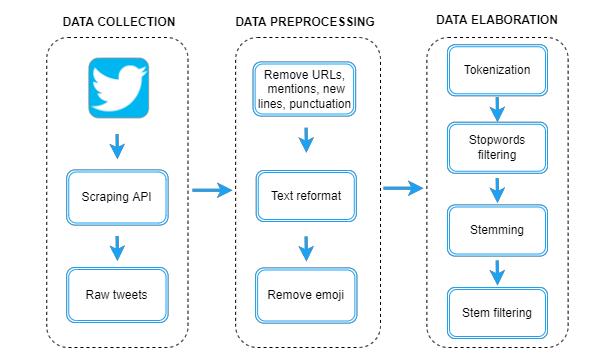
\includegraphics[width=0.8\textwidth]{images/dataset/preprocessing.png} 
    \caption{Data fetching and preprocessing} 
    \label{fig:preprocessing}
\end{figure}




